% sample file for Modelica Conference paper

\documentclass[11pt,a4paper,twocolumn]{article}
\usepackage{graphicx}
\graphicspath{{fig/}}
\usepackage[T1]{fontenc}
\usepackage[british]{babel}      % some british specific settings
\usepackage[utf8]{inputenc}    %% european characters can be used
\usepackage{lmodern,amsmath,mathptmx,url}      %% recommended for readable pdf
\pagestyle{empty}                %% no page numbers!
\usepackage{geometry}            %% please don't change geometry settings!
\geometry{left=20mm, right=20mm, top=25.4mm, bottom=25mm, noheadfoot, columnsep=8mm}
\parindent0pt
\bibliographystyle{ieeetr}

% some additional packages
\usepackage{listings} % for code listings
\usepackage{color}

% usefull commands
\newcommand{\myr}{\textsuperscript{\textregistered}}
\newcommand{\ud}{\mathrm{d}}
\newcommand{\matx}[1]{\mathbf{#1}}
\newcommand{\impact}{\texttt{impact.py}}

\begin{document}

\title{\textbf{{\small Modelica'2014}\\
    \texttt{impact.py} -- A Modelica\myr\ Package Manager}}

\author{Michael Tiller\\Xogeny Inc., USA\\\url{michael.tiller@xogeny.com} %
        \and Dietmar Winkler\\Telemark University College, Norway\\\url{dietmar.winkler@hit.no}}
\date{} % <--- leave date empty
\maketitle\thispagestyle{empty} %% <-- you need this for the first page

\section*{Abstract}
%TODO


\paragraph{Keywords:}\emph{modelica, package manager, github, dependency management}

\section{Introduction}
\label{sec:intro}
%TODO
In Fig.~\ref{fig:newtons_cradle} you see a possible candiate for a logo.


\begin{figure}[!ht]
  \centering
  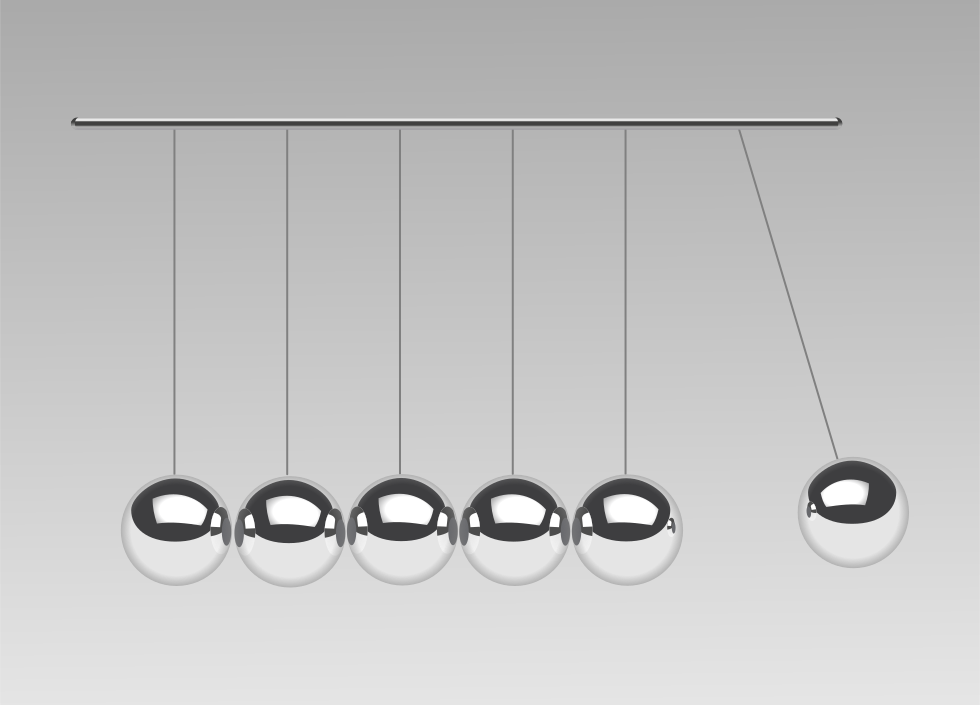
\includegraphics[width=\columnwidth]{newtons_cradle}
  \caption{Possible logo candidate \cite{Andersson2007}}
  \label{fig:newtons_cradle}
\end{figure}


\section{Background}
\label{sec:background}

Problems we want to solve:
\begin{itemize}
\item one
\item another one
\item and a third one
\end{itemize}


\subsection{Exisiting solutions}
\label{sec:exist-sol}

\subsection{New approach}
\label{sec:exist-sol}
Foo
\lstset{language=python}
\begin{lstlisting}[frame=single]  % Start your code-block

from setuptools import setup

setup(name="impactlib",
      version="0.1.0",
      description="Modelica package manager",
      author="Michael Tiller",
      author_email="michael.tiller@gmail.com",
      url="http://www.xogeny.com/",
      scripts=['scripts/impact.py'],
      packages=['impactlib'])
\end{lstlisting}


Search for librararies is done by executed by doing:
\lstset{language=bash}
\begin{lstlisting}[frame=shadowbox]  % Start your code-block

impact.py search <search term>
\end{lstlisting}

\section{Discussion}
\label{sec:discussion}
%TODO

\section{Conclusion}
\label{sec:conclusion}
%TODO

\bibliography{impact}
\end{document}
